%%%%%%%%%%%%%%%%%%%%%%5
\graphicspath{{}{nustorm/}{Diagrams/}}


This chapter is dedicated to studying sterile neutrinos in short-baseline oscillations, and discusses two well-known but distinct types of non-unitarity. As a novelty, we investigate these effects with the experimental proposal of Neutrinos from STORed Muons ($\nu$STORM). \nus is a proposal for a non-conventional but well-understood neutrino beam from the decay of stored muons. The energy range and the sub-percent uncertainties on the neutrino flux make \nus a precision facility with GeV neutrinos. On top of its importance as a first step towards large scale muon facilities (\eg, neutrino factories~\cite{Choubey:2011zzq} and muon colliders), the project is very timely as it would provides precise measurements of neutrino-nucleus cross sections. This would serve as an input for long-baseline physic~\cite{Soler2015}, increasing the sensitivity of future experiments to CP violation and other oscillation parameters. The key step ingredient for this project lies in the precise knowledge of the flux, disentangling for the first time the knowledge of the flux from that of the cross sections. In this way, \nus also provides a clean and intense environment to search for new physics~\cite{Adey:2013pio,Adey:2014rfv,Ballett:2017bug}. In this chapter, we will explore a \nus setup with two iron-scintillator detectors, resembling the original proposal for siting at Fermilab, using 60 GeV protons~\cite{Adey:2013pio} and $3.8$ GeV stored muons. At the time of writing, the Fermilab design is currently being reconsidered for siting at CERN instead. While the details of the new proposal are uncertain, it is likely to incorporate larger muon energies (up to $E_\mu \lesssim 6$ GeV) and reviewed detector options~\cite{Long:2018zpc}.


In this chapter we discuss sterile neutrinos in the most minimal extension of the SM by the neutrino portal. Although the scale of the new state is arbitrary, we would like to focus on light states which can be probed in laboratory. We adopt a pure phenomenological approach, and refrain from connecting such steriles to neutrino mass generation. In particular, we consider steriles from sub-eV masses to arbitrarily heavy states. The interest in the eV scale arises from the series of experimental anomalies at short baselines (see Refs.~\cite{Diaz:2019fwt} and~\cite{Dentler:2018sju} for a review on this topic). For instance, the excess of $\nu_e$-like events in a beam of predominantly $\nu_\mu$ states at the Liquid Scintillator Neutrino Detector (LSND)~\cite{Aguilar:2001ty} and at the MiniBooNE experiment~\cite{Aguilar-Arevalo:2018gpe}. Other short-baseline anomalies exist also in the form of a deficit of $\nu_e$ and $\overline{\nu}_e$ states in radioactive source experiments~\cite{Hampel:1997fc,Abdurashitov:2005tb}, as well as in reactor experiments~\cite{Mention:2011rk}. It is intriguing, however, that these results are in severe conflict with null-results from $\nu_\mu \to \nu_\mu$ experiments, such as MINOS~\cite{Adamson:2017uda} and IceCUBE~\cite{TheIceCubeCollaboration2016}. The tensions between datasets in an eV sterile neutrino interpretation of these anomalies are large. For this reason, we also refrain from connecting our discussion to such anomalies. Nevertheless, searching for steriles and non-unitarity of the PMNS matrix is a worthwhile goal of next generation experiments. This topic may also receive high priority in case of future positive results from the currently running $\mu$BooNE~\cite{Adams:2019iqc} experiment, as well as from the full short-baseline program (SBN) currently under construction at Fermilab~\cite{Cianci2017}. \nus would offer a robust and unique chance to study eV-scale sterile neutrinos using $\nu_e \to \nu_\mu$ appearance, rather than through $\nu_\mu \to \nu_e$ appearance studied by all other experiments.


\section{Short-Baseline Oscillations}
%
Standard Model neutrinos produced in charged current interactions are flavour eigenstates $\nu_{\alpha}$ ($\alpha = e,\mu$ or $\tau$). The misalignment between the flavour eigenstates $\ket{\nu_{\alpha}}$ and the mass eigenstates $\ket{\nu_i}$ in the presence of non-degenrate masses is responsible for neutrino oscillations and mixing. The mixing is described by a matrix $U$, which in the case of 3 active neutrinos is given by the $3 \times 3$ Pontecorvo-Maki-Nakagawa-Sakata (PMNS) matrix. In general, for $3+N$ flavour and $3+N$ mass eigenstates, we have
%
\begin{equation} \label{eq:mixing}
\ket{\nu_{\alpha}} = \sum_{i}^{3+N} U_{\alpha i}^* \ket{\nu_{i}}.
\end{equation}   
%
The invisible decay width of the Z boson as measured at LEP \cite{Schael2006} indicates that there are only 3 weakly interacting neutrino states. The $N$ additional flavour eigenstates will be referred to as sterile states, as these are singlets under all SM gauge groups. Similarly, the $N$ additional mass eigenstates are also typically called sterile, since that is their dominant flavour composition.

In general, in a quantum mechanical treatment of neutrino oscillations, the oscillation probability for a neutrino preoduced as a flavour $\alpha$ to be detected as a state $\beta$ can be written as a function of the baseline $L$ and the neutrino energy $E$ as
%
% \begin{equation} \label{eq:general_prob}
% P_{{\alpha {\beta}}}(L, E) = \sum_{j}^{3+N} \sum_k^{3+N} U_{\alpha j}^* U_{\beta j} U_{\alpha k} U_{\beta k}^* \, I_{j k} (L, E),
% \end{equation}    
%
\begin{align} \label{eq:general_prob}
P_{\nu_{\alpha} \to \nu_{\beta}}= \delta_{\alpha \beta} -& 2 \sum_{k>j}^{3+N} \Re(U_{\alpha k}^* U_{\beta k} U_{\alpha j} U_{\beta j}^*)\, \left(1 - \Re\left[I_{k j}(L, E)\right]\right) \nonumber\\ -& 2\sum_{k>j}^{3+N} \Im(U_{\alpha k}^* U_{\beta k} U_{\alpha j} U_{\beta j}^*) \Im\left[I_{k j}(L, E) \right],
\end{align}
where the factor $I_{k j}(L, E)$ satisfies $I_{k k} = 1$ and $I^*_{k j} = I_{j k}$ \cite{Akhmedov2009} and will contain any information about the coherence of production, propagation and detection of neutrino mass states. More commonly, under the plane-wave approximation and assuming ultra-relativistic neutrinos with $L = t$, this factor is related to the time evolution of the mass eigenstates and reads
%
\begin{equation} \label{eq:Iplanewave}
I_{k j}(L, E) = \exp\left(-i \frac{\Delta m^2_{k j} L}{2 E}\right).
\end{equation}
%
The plane-wave approximation, however, fails to properly accommodate effects due to the finite size of the production or detection region, which might play an important role in oscillations due to steriles with masses above a few eV. In section \ref{sec:prodcoh} we motivate and lay out the necessary formalism developed in \cite{Akhmedov2009,Akhmedov2012} for dealing with these issues.

Equation \ref{eq:mixing} implies that with the addition of $N$ sterile neutrinos the mixing matrix is enlarged to an $N \times N$ matrix. At the short-baselines we are interested in, however, we can safely ignore any terms in the oscillation probability which contain the active mass-squared differences ($\Delta m^2_{31} \approx 7 \times 10^{-5}$ eV$^2 \ll\Delta m^2_{21} \approx 10^{-3}$ eV$^2 \ll \Delta m^2_{\text{SBL}}$). All oscillations (as a special case of flavour transitions) discussed in this paper will be due to active-sterile mass-squared differences $\Delta m^2_{\text{SBL}}$, which are taken to be in the range $10^{-1}$ -- $10^{3}$ eV$^2$. In particular, we will only consider the case where all sterile neutrinos are heavier than the active ones.   

In a 3+1 scenario under the short-baseline approximation, equation \ref{eq:general_prob} gives the following oscillation probability
%
\begin{equation} \label{eq:app3+1}
P^{3+1}_{\nu_{\alpha} \to \nu_{\beta}} = 2 |U_{\alpha 4}|^2 |U_{\beta 4}|^2 \big(1 -\Re(I_{41}) \big)
\end{equation}
%
for appearance, and
%
\begin{equation} \label{eq:dis3+1}
P^{3+1}_{\nu_{\alpha} \to \nu_{\alpha}} = 1 - 2|U_{\alpha 4}|^2(1 - |U_{\alpha 4}|^2) \big(1 -\Re(I_{41}) \big),
\end{equation}
%
for disappearance. In the 3+1 case, it is customary to write the probabilities in terms of the more phenomenological parameters $\sin^2 {2 \theta_{\alpha \beta}} = 4 |U_{\alpha 4}|^2 |U_{\beta 4}|^2 $ and $\sin^2 {2 \theta_{\alpha \alpha}} = 4 |U_{\alpha 4}|^2(1 - |U_{\alpha 4}|^2) $, and we use these througout the paper.

In the presence of two sterile neutrinos at the eV scale, the oscillation is effectively a 3 neutrino case. This means that the probability formula picks up a complex phase, which will be parametrized by $\eta = \arg{(U_{\alpha 5}^* U_{\beta 5} U_{\alpha 4} U_{\beta 4}^*)}$. The short baseline approximation to the probability reads
%
\begin{align}
P^{3+2}_{\nu_{\alpha} \to \nu_{ \beta}}  =\, &2 \left|U_{\alpha 4}\right|^2 \left|U_{\beta 4}\right|^2 \left(1 - \Re(I_{4 1}) \right) + 2 \left|U_{\alpha 5}\right|^2 \left|U_{\beta 5}\right|^2 (1 - \Re(I_{5 1})) \nonumber \\
+ &2 \left| U_{\alpha 4} U_{\beta 4} U_{\alpha 5} U_{\beta 5}\right|  \Re\left[ e^{i \eta} \left( 1 - I_{41}^* - I_{51} + I_{54} \right) \right],
\end{align}
%
for apperance, and
%
\begin{align}
P^{3+2}_{\nu_{\alpha} \to \nu_{ \alpha}}  =\,1 - &2(1 - |U_{\alpha 4}|^2 - |U_{\alpha 5}|^2) \times \left[ |U_{\alpha 4}|^2 \big(1 - \Re(I_{41}))  + |U_{\alpha 5}|^2 \big( 1 - \Re(I_{51}) \big)\right] \nonumber \\ - &2 |U_{\alpha 4}|^2 |U_{\alpha 5}|^2 \left(1 - \Re(I_{54})\right), 
\end{align}
%
for disappearance. Note how the CP complex phase only appears in the appearance formulae since CPT invariance implies CP conservation for the disappearance channel. Full expressions for the oscillation probability in the plane wave approximation can be obtained by using \refeq{eq:Iplanewave}, and for production decoherence assuming point-like parent particles one can use the expressions for $I_{k j}$ we discuss below.

%%%%%%%%%%%%%%%%%%%%%%%%%%%%%%%%%%%%%%%%%%%%%%%%%%%%%%%%%%%%%%%%%%%%%%%%%%% 
\subsection{Localization at Production \label{sec:prodcoh}}

The presence of light sterile neutrinos with masses above the eV scale can realise the interesting scenario where the localization at production might be broken. For a neutrino to be created as a coherent superposition of different mass eigenstates we should not be able to resolve what mass eigenstate was produced, {\it i.e.} $\sigma_{m^2} \gg \Delta m^2$ for all the involved mass-splittings is a condition for production coherence~\cite{Akhmedov2012}. Using the relativistic expression for the neutrino energy, the condition for the uncertainty on the neutrino momentum $\sigma_P$ can be written as
%
\begin{equation}
\sigma_P \gg \frac{\Delta m^2}{2P}.
\end{equation}
%
If we assume that $\sigma_P$ is related to the uncertainty in the spatial coordinate of the neutrino as $\sigma_P \sim \text{\it min} (1/\sigma_{x_S}, 1/\sigma_{x_D})$, we arrive at the well known condition for neutrino oscillations not to be washed-out \cite{Akhmedov2009}
%
\begin{equation}
\sigma_{x_S} \ll L_{\text{osc}}, \quad \sigma_{x_D} \ll L_{\text{osc}},
\end{equation} 
%
where $L_{\text{osc}} = 4 \pi P/\Delta m^2$ and factors of 2 and $\pi$ were ignored. This condition says that the production or detection decoherence effects are equivalent to the averaging of the oscillations due to finite size of sources and detectors.

The production region at $\nu$STORM, for example, is given by the size of the decay pipeline $\ell_p = 180$ m. This is only an order of magnitude smaller than the far detector baseline ($\approx 2$ km) and, more importantly for higher mass sterile searches, it is larger than the near detector distance from the end of the decay pipeline. For instance, if a sterile neutrino with a mass larger than $10$ eV is present, the near detector would only see flavour transitions constant in energy.

The probabilities derived in the previous section have been derived for a general factor $I_{k j}$, which under the plane-wave approximation is given by equation \ref{eq:Iplanewave}. In the wavepacket treatment for neutrino oscillations, $I_{k j}$ is corrected by production, detection and propagation coherence factors \cite{Akhmedov2009}:
%
\begin{equation}
I_{k j} = \exp\left(-i \frac{\Delta m^2_{k j} L}{2 P}\right) S_{\text{prop}}(L/L^{\rm coh}_{kj}) S_{\text{P/D}}(\sigma_x/L^{\rm osc}_{k j}),
\end{equation}
%
where the $S$ damping factors are due to propagation coherence, and localization at production and detection. The quantity $L^{\rm coh}_{kj}= 4\sqrt{2} E^2 \sigma_x /|\Delta m^2_{kj}|$ is the coherence lenght of a pair of mass eigenstates, \textit{i.e.} the lenght in which the two states continue to have a significant overlap of their coordinate wave packets. The $S$ factors are equal to unity for zero arguments and quickly decrease for increasing arguments. In this study, we ignore any propagation and detection effects and focus only on the production localization $S_{P}$. We choose to work with the formalism developed in references~\cite{Hernandez2011,Akhmedov2012}, where oscillation probabilities were derived in the quantum mechanical wavepacket approach. This approach is in contrast with the incoherent summation of the probability along the production region, where the straight averaged neutrino flux is given by a convolution of the plane wave probability formula and the neutrino flux at different points of the decay straight. The equivalence of the two approaches is discussed in Ref.~\cite{Akhmedov2012}, and for all our purposes they lead to the same results as long as the neutrino parent particles can be treated as pointlike, \emph{i.e.} have vanishingly small wavepacket spatial width. It should be emphasized, however, that the wavepacket formalism is more general than the incoherent probability summation. Moreover, the available neutrino fluxes for \nus already take the finite size of the production region into account~\cite{Tunnell2013}, and cannot be convolved with the oscillation probability over the production region once more.

Finally, let us emphasize our results are robust against different estimates for the neutrino wavepacket. If it turns out to be smaller than the production region, due to collisions of the parent partcles with the residual gas in the decay pipe, for instance, then our results remain unchanged. This is because even in this scenario, the production region is large, and the classical avereging of the probability over it leads to the washing out of the oscillation. This is, again, a reflection of the fact that our formalism is analogous to the incoherent summation of the probability over the production region. If, instead, the wavepacket is larger, due to large parent particle wavepacket size, for instance, then corrections to our method are in place. In this case, additional averaging effects would be at play, suppressing oscillations with large $\Delta m^2$.

Expressions for the $S_P$ factors as well as the full oscillation probabilities for some channels are given below. For completeness, we show the $I_{k j}$ factors that have been used in our calculations, corresponding to the case of pointlike parent particles and pontlike detection approximations derived in~\cite{Akhmedov2009}. For clarity, we omit all $k\,j$ mass subscripts in our expression, leaving only indices corresponding to the neutrino parent particle $X = \mu, \pi$. We write it in two forms: a compact formula, and one in which the real and imaginary parts are explicitly separated: 
%
\begin{align}\label{eq:Ijk}
I_{k j} = \, & \frac{1}{1 - e^{-\sfrac{\Delta_p}{\xi_X}}} \frac{1}{1 - i\xi_X} \left[ 1  - e^{-\sfrac{\Delta_p}{ \xi_X} } e^{i  \Delta_p}\right] e^{-i \Delta}\nonumber \\
= \, & \frac{1}{1 - e^{-\sfrac{\Delta_p}{ \xi_X} }} \frac{1}{1 + \xi^2_X} \biggr\{ \cos{\Delta} + \xi_X \sin{\Delta} - e^{-\sfrac{\Delta_p}{ \xi_X}} \big( \cos{(\Delta- \Delta_p)} + \xi_X \sin{(\Delta - \Delta_p)}\big) + \nonumber\\
&\quad \quad i \left[ \xi_X \cos{\Delta} - \sin{\Delta} - e^{-\sfrac{\Delta_p}{ \xi_X}} \big( \xi_X \cos{(\Delta - \Delta_p)}  - \sin{(\Delta - \Delta_p)} \big) \right]   \biggr\}.
\end{align}
%
In the expression above we denote the lenght of the decay pipeline by $\ell_p$ and use the following definitions:
\begin{align}
\Delta = \frac{\Delta m^2_{k j}}{2P}L, \quad \Delta_{p} = \frac{\Delta m^2_{k j}}{2P} \ell_p,\quad \xi_X = v_{X} \frac{\Delta m^2_{k j}}{2P}\ell_{\text{dec}_X},
\end{align}
where the parent particle properties enter our probability formulas via $\xi_X$ with the velocity $v_{X}$ and the decay lenght $\ell_{\text{dec}_X} = 1 / \Gamma _X$.

Using the definitions above and the $I_{k j}$ factor in \refeq{eq:Ijk}, we can write the probability formulas for our 3+N models. As an example, we show the 3+1 apperance and disapperance formulas of interest, choosing  $\sin^2{2 \theta_{e \mu}} = 4 |U_{e \mu}|^2 |U_{\mu \mu}|^2$ and $\sin^2{2 \theta_{\mu \mu}} = 4 |U_{e \mu}|^2 (1 - |U_{\mu \mu}|^2)$. For appearance, it reads
%
\begin{align} \label{eq:probApp3+1}
P^{3+1}_{\nu_{e} \to \nu_{\mu}} = \sin{2 \theta_{e \mu}} \bigg\{1 &- \frac{1}{1 - e^{-\sfrac{\Delta_p}{ \xi_X} }} \frac{1}{1 + \xi^2_X} \Big[ \cos{\Delta} + \xi_X \sin{\Delta} \nonumber \\  &- e^{-\sfrac{\Delta_p}{ \xi_X}} \big( \cos{(\Delta- \Delta_p)} + \xi_X \sin{(\Delta - \Delta_p)}\big) \Big] \bigg\},
\end{align}
%
while for disappearance, 
\begin{align}
P^{3+1}_{\nu_{\mu} \to \nu_{\mu}} = \sin^4{\theta_{\mu \mu}}+\cos^4{\theta_{\mu \mu}} &+ \frac{\sin^2{2 \theta_{\mu \mu}}}{1 - e^{-\sfrac{\Delta_p}{ \xi_X} }}  \frac{1}{1 + \xi^2_X} \bigg[ \cos{\Delta} + \xi_X \sin{\Delta} \nonumber \\ &- e^{-\sfrac{\Delta_p}{ \xi_X}} \big( \cos{(\Delta- \Delta_p)} + \xi_X \sin{(\Delta - \Delta_p)}\big) \bigg].
\end{align}
%

\subsection{Non-Unitarity from Light and Heavy Sterile Neutrinos}
%

The scale of the new sterile state is completely arbitrary from a theoretical point of view, each one with its own distinct phenomenology. At most oscillation experiments, however, any sterile neutrino with a mass above $\mathcal{O}(10)$ eV leads to what we call an effective \emph{zero-distance} effect, whether through its averaged-out oscillations or due to integrating out the heavy states. In the following, we will have a glimpse these two regimes. In all our discussion we will neglect the decay of the heavy states, although we note that extra interactions of the new states trying to reconcile cosmology and sterile neutrinos might decrease its lifetime~\cite{Mirizzi2014,Chu2015,Archidiacono2014,Archidiacono2016}. 

It is instructive to divide the parameter space into three regions.
%
\begin{itemize}
 \item The sterile neutrino is kinematically accessible and can be produced in muon or pion decays, but its oscillation lenght is too small to be seen at any reasonable experiment.
 \item The sterile mass is close to but still smaller than the parent particle mass and impacts the neutrino production and detection rate due to kinematical factors. This intermediate region is relevant for meson decay peak searches, but less important for oscillation experiments.
 \item The sterile is much heavier than the parent particle and cannot be produced at the oscillation experiments. This is effectively identical to integrating out the heavy state.
\end{itemize}
%
There is no fundamental difference between the first two scenarios, except that in the first one the effects due to the mass of the sterile are too small to be relevant. The third case concerns masses above the electroweak scale, and is typically studied under the minimal unitarity violation (MUV) formalism~\cite{Antusch2006}. In an effective field theory, one can parametrize the effects of these large mass steriles via the non-unitarity of the PMNS matrix. One can show that this arises from the non-orthonormality of the low-scale flavour states at oscillation experiments. 

We will aim at connecting the high-scale non-unitarity and the averaged out oscillations of light steriles. First, however, we will explore where the zero-distance effects are coming from in the two cases. Later, by trying to be as general as possible in the derivation of the event rates, we will attempt to develop a formalism that explicitly shows how these effects change at different mass scales. 

\subsubsection{Averaged-Out Steriles} First, we will explore the phenomenology of sterile neutrinos above the eV scale but lighter than their parent particles. Once the sterile mass is too large to allow for oscillation with active neutrinos to happen (\eg, due to production localization effects) the sterile states contribute to the oscillation probability only through a constant term. This contribution stems from the fact that even in the absence of oscillations, flavour transitions are still possible. This regimes comprises masses of $10 \, \text{eV}\, \lesssim m_{4} < m_{\mu} (m_{\pi})$. 

If we neglect any effects on the neutrino production due to the sterile mass, and take the limit of $L \ll L^{\text{osc}}_{k j}$ (or $\sigma_x \ll L^{\text{osc}}_{k j}$), we get
%
\begin{align}
 P_{\nu_{\alpha} \to \nu_{\beta}} &= \sum_{k}^{3+N} |U_{\alpha k}|^2|U_{\beta k}|^2 + 2 \sum_{k > j}^{3}\Re{\left( U^*_{\alpha k} U_{\alpha j} U_{\beta k} U^*_{\beta j} \right)}, \nonumber \\
 &= \left| \sum_{k}^{3} U_{\alpha k}^* U_{\beta k} \right|^2 + \sum_{k=3+1}^{3+N} |U_{\alpha k}|^2 |U_{\beta k}|^2,
\end{align}
%
where we averaged out active-sterile phases to zero and kept all active terms for which $L \ll L^{\text{osc}}_{k j}= 4 \pi E / \Delta m^2_{k j}$. In a 3+1 model, for instance, one can reduce this expression using the unitarity of the mixing matrix $\sum_k^{3+1} U_{\alpha k} U_{\beta k}^* = \delta_{\alpha \beta}$ to
%
\begin{equation}
 P_{\nu_{\alpha} \to \nu_{\beta}} = 2 |U_{\alpha 4}|^2 |U_{\beta 4}|^2,\quad P_{\nu_{\alpha} \to \nu_{\alpha}} = 1 - 2 |U_{\alpha 4}|^2 + 2|U_{\alpha 4}|^4,\label{eq:AOS3+1dis}
\end{equation}
%
for appearance and disappearance, respectively. The interpretation of the appearance formula is clear: the constant oscillation probability only provides the mixing factor required to obtain the flux of sterile states from the flux of $\nu_{\alpha}$ at production and another mixing factor to obtain the probability that such a state interacts as a neutrino of flavour $\beta$. The zero-distance effects in this case is given by the possibility that the sterile state is produced, propagates ballistically to the detector and scatters off a nuclei creating another flavour lepton.

\subsubsection{Integrated-Out Steriles} In this section we summarize the main results of Ref.~\cite{Antusch2006}. The mixing amongst active neutrinos is given by the sub-block $N$ of the neutrino mixing matrix $U$, such that the flavour neutrino fields are given by
\begin{equation}
 \nu_{\alpha} = \sum_i ^{3} N_{\alpha i} \, \nu_i, \quad \text{where} \quad U = \left(\begin{matrix} N & \Theta \\ R & S\end{matrix} \right).
\end{equation}
Here, $U$ is the full unitary mixing matrix of neutral leptons, and $N$ the non-unitary PMNS matrix describing the mixing of active-light states. $R$, $S$ and $\Theta$ contain the mixing between active-heavy, sterile-heavy and sterile-light states, respectively, and are also not unitary in general. Note that the orthonormality of the neutrino mass states still holds, but the quantum states associated to neutrinos of a specific flavour (like the state produced from the decay of a pion or a muon) are no longer formed by a complete basis, and are no longer orthonormal. The true flavour states are orthonormal, but they require the presence of the heavy neutrino state, which is not produced in terrestrial oscillation experiments. Additional normalization factors are then necessary for the flavour state produced
\begin{equation}
 \ket{\nu_{\alpha}} = \frac{1}{\sqrt{(NN^{\dagger})_{\alpha \alpha}}} \sum_{i}^{3} N_{\alpha i}^* \ket{\nu_i},
\end{equation}
where for a 3+1 model, for example, would yield $(NN^{\dagger})_{\alpha \alpha} = 1 - |U_{\alpha 4}|^2$. This normalization factor appears in the calculation of the oscillation probability as
\begin{equation}
 P_{\nu_{\alpha} \to \nu_{\beta}} = \frac{\left| \sum_{i}^3 N_{\alpha i}^* e^{-i P_i L} N_{\beta i} \right|^2}{(NN^{\dagger})_{\alpha \alpha} (NN^{\dagger})_{\beta \beta}},
\end{equation}
which at zero-distance ($L=0$, before active oscillations take place) is
\begin{equation}
 P_{\nu_{\alpha} \to \nu_{\beta}} = \frac{\left| (NN^{\dagger})_{\beta \alpha} \right|^2}{(NN^{\dagger})_{\alpha \alpha} (NN^{\dagger})_{\beta \beta}}.
\end{equation}
This is not the end of the story, however, as the neutrino production and detection also receive corrections due to the non-unitarity of the mixing matrix. In particular, the following relations are valid for charged current processes (CC) with a single neutrino involved
\begin{equation}
 \sigma_{\alpha}^{\text{CC}} =  \sigma_{\alpha}^{\text{CC (SM)}} (NN^{\dagger})_{\alpha \alpha}, \quad \frac{ d\Phi^{\text{CC}}_{\beta}}{dE} = \frac{ d\Phi^{\text{CC (SM)}}_{\beta}}{dE} (NN^{\dagger})_{\beta \beta},
\end{equation}
whilst for CC processes with two neutrino flavours (\textit{e.g.}, muon decay) receive additional corrections
\begin{equation}
 \sigma_{\alpha}^{\text{CC}} =  \sigma_{\alpha}^{\text{CC (SM)}} (NN^{\dagger})_{\alpha \alpha}(NN^{\dagger})_{\beta \beta}, \quad \frac{ d\Phi^{\text{CC}}_{\beta}}{dE} = \frac{ d\Phi^{\text{CC (SM)}}_{\beta}}{dE} (NN^{\dagger})_{\alpha \alpha} (NN^{\dagger})_{\beta \beta}.
\end{equation}
Neutral current processes also receive corrections, but of the type $|(NN^{\dagger})_{i j}|^2$. The previous expressions hint at a cancellation between the normalization factors in the probability and the corrections to the production and detection. This means that at an oscillation experiment neutrinos from pion decay would not be affected by the normalization factors, whilst neutrinos from muons could. In addition, the oscillation probability differs from the averaged out one, even when the cancellations are in place. We can see that by comparing the quartic term in the following 3+1 probability with the one in the previous section (\refeq{eq:AOS3+1dis})
\begin{equation}
 P_{\nu_{\alpha} \to \nu_{\beta}} = \frac{\left| \delta_{\alpha \beta} - U_{\alpha 4}^*U_{\beta 4} \right|^2}{(1-|U_{\alpha 4}|^2)(1-|U_{\beta 4}|^2)} %
 = \frac{ \delta_{\alpha \beta} - 2 \delta_{\alpha \beta} |U_{\alpha 4}|^2 + |U_{\alpha 4}|^2 |U_{\beta 4}|^2}{(1-|U_{\alpha 4}|^2)(1-|U_{\beta 4}|^2)}.
\end{equation}

For completeness, we also show the parameterizations for the non-unitarity of the mixing matrix $N$ used in the literature. For instance, Ref.~\cite{Blennow:2016jkn} chooses to use a lower triangular matrix $\boldsymbol{\alpha}$ as in
\begin{equation}
 N = (\boldsymbol{1} - \boldsymbol{\alpha}) U,
\end{equation}
where $U$ is the analogue of the PMNS matrix and unitary and 
\[
\boldsymbol{\alpha} =
  \begin{pmatrix}
    \alpha_{e e} & 0 & 0 \\
    \alpha_{\mu e} & \alpha_{\mu \mu} & 0 \\
    \alpha_{\tau e} & \alpha_{\tau \mu} & \alpha_{\tau \tau} \\
  \end{pmatrix},
\]
with real diagonal entries. Using the previous parametrization one can then write the quantity of interest $NN^{\dagger}$ (omitting the tau entries) as 
%
\begin{equation}
 NN^{\dagger} = \boldsymbol{1} - \boldsymbol{\alpha} - \boldsymbol{\alpha}^{\dagger} + \boldsymbol{\alpha}\boldsymbol{\alpha}^{\dagger} =\begin{pmatrix}
    1 - 2\alpha_{e e} +\alpha_{e e}^2 & \alpha_{\mu e}^*(\alpha_{ee}-1) & * \\
    \alpha_{\mu e}(\alpha_{ee}-1) & 1 - 2\alpha_{\mu \mu} + \alpha_{\mu \mu}^2 + |\alpha_{\mu e}|^2 & * \\
    * & * & * \\
  \end{pmatrix}.
\end{equation}
%
Alternatively, one can parametrize $N$ as $N = \boldsymbol{T} U$, where we use the matrix $\boldsymbol{T}$ from Ref.~\cite{Escrihuela2015}, which is written as
%
\begin{equation}
\boldsymbol{T} =
  \begin{pmatrix}
    \alpha_{11} & 0 & 0 \\
    \alpha_{21} & \alpha_{22} & 0 \\
    \alpha_{31} & \alpha_{32} & \alpha_{33} \\
  \end{pmatrix}.
\end{equation}
%
In this parametrization, the quantity of interest $NN^{\dagger}$ is slightly simpler
\begin{equation}
NN^{\dagger} =
  \begin{pmatrix}
    \alpha_{11}^2 & \alpha_{11}\alpha_{21}^* & * \\
    \alpha_{11}\alpha_{21} & \alpha_{22}^2 + |\alpha_{21}|^2 & * \\
    * & * & * \\
  \end{pmatrix},
\end{equation}
and the relation between the two parametrizations is clear: $\alpha_{\alpha \beta} \to \delta_{ij} - \alpha_{ij}$, with $e \to 1, \mu \to 2$ and $\tau \to 3$. Bounds on the non-unitarity parameters can be derived from a variety of processes and have been collected in Refs.~\cite{Fernandez-Martinez:2016lgt}, for instance.

\subsubsection{Understanding the Gap}

In this section we will connect the two regimes described above at the level of oscillation probabilities. For the sake of our argument, a plane wave treatment is sufficient. We begin with a neutrino flavour state produced in the interaction  $P_I \to P_F \, \ell^+_{\alpha} \, \nu_{\alpha}$, written as
\begin{equation}\label{eq:general_flavor_state}
\ket{\nu_{\alpha}} = \frac{1}{\sqrt{\sum_i \left|A_{\alpha i}\right|^2}} \sum_k^{3+N} A_{\alpha k} \ket{\nu_{k}},
\end{equation}
where the amplitude for producing a neutrino mass eigenstate is given by 
\begin{equation}
A_{\alpha k} = \bra{\nu_k , \ell^+_{\alpha} , P_F} \hat{S} \ket{P_I} = U_{\alpha k}^* \mathcal{F}_{k} M_{\alpha}. \label{eq:amplitude}
\end{equation}
Here we factorised the amplitude for neutrino production into a mixing matrix element $U_{\alpha k}$, a factor $\mathcal{F}_k$ containing all the dependence on the neutrino mass $m_k$, and the remaining flavour-dependent factor $M_{\alpha}$. Just remains an \emph{assumption} in what follows. More concretely, the factor $\mathcal{F}$ can be thought of as a kinematical factor in the calculation of the neutrino production and detection, and carries information about the heavy neutrino mass and its ratio to the other scales involved. In writing the equation above, we are assuming that the matrix element $M_\alpha$ has no dependence on the neutrino mass~\footnote{While this is customary for $\mathcal{F}^P$, which can be thought of as a Shrock factor~\cite{Shrock:1980ct} in meson decay processes, $\mathcal{F}^D$ requires more care due to the more complex nature of the scattering process.}. Within our assumptions, $\mathcal{F}_k = 1$ when $m_k \ll M_P$, where $M_P$ is the mass of the parent particle of the neutrino, and $\mathcal{F}_k = 0$ when $m_k > M_P$. The amplitude for the production of a neutrino of specific flavour is then
%
\begin{equation}
\left| A_{\alpha} \right|^2 = \sum_k \left| U_{\alpha k} \right|^2 \left| \mathcal{F}_k \right|^2 \left| M_{\alpha} \right|^2.
\end{equation}     
%
When only one heavy neutrino is present and all light states have $\mathcal{F}_k = 1$ for $k < 4$, we can write
%
\begin{align}
\left| A_{\alpha} \right|^2 &= \left( \sum_k^3 \left| U_{\alpha k} \right|^2 + |U_{\alpha 4}|^2 \left| \mathcal{F}_4 \right|^2 \right)\left| M_{\alpha} \right|^2  = \left( 1 + \left( |\mathcal{F}_4|^2 - 1 \right) |U_{\alpha 4}|^2 \right) \left| M_{\alpha} \right|^2  
\end{align}     
reducing to
\begin{equation}
|A_{\alpha}|^2 = |M_{\alpha}|^2,
\end{equation}
for averaged-out steriles, and
\begin{equation}
|A_{\alpha}|^2 = \left( 1 - |U_{\alpha 4}|^2 \right)|M_{\alpha}|^2,
\end{equation}
for integrated-out steriles. The neutrino flux, which is proportional to $|A_{\alpha}|^2$, receives similar corrections. A very similar discussion can be made for the amplitude of detection, where we will now call $\mathcal{F}^P_k$ and $\mathcal{F}^D_k$ the kinematical factor for the production and detection state, respectively.

We will now calculate the flavour transition probability assuming that the fourth mass eigenstate is heavy enough that it will not oscillate, allowing only for zero-distance effects. We start by defining general flavour states as in \refeq{eq:general_flavor_state} for production and detection, $ \ket{\nu_{\alpha}^P}$ and $\ket{\nu_{\beta}^D}$. Expanding the amplitude as in \refeq{eq:amplitude}, we obtain the production state
\begin{align}
\ket{\nu_{\alpha}^P} &=  N^{P}_\alpha \, \hat{M}_{\alpha}^P \,\sum_i^{3+N} U_{\alpha i}^* \mathcal{F}^P_i \ket{\nu_{i}},
\end{align}
where $\hat{M}_{\alpha}^P = M_{\alpha}^P / |M_{\alpha}^P|$ and $\left(N^{P}_\alpha\right)^{-2} = {\sum_{i}^{3+N} \left|U_{\alpha i} \mathcal{F}_i^{P}\right|^2 }$. An analogous expression is valid for the detection state. When calculating the oscillation probability, we will need the transition amplitude
%
\begin{align}
\mathcal{A}_{\alpha \to \beta} =&  \bra{\nu_{\beta}^D} e^{- i \hat{E} T + i \hat{p} L} \ket{\nu_{\alpha}^P} = N^{P}_\alpha N^{D}_\beta \, \hat{M}_{\alpha}^P \hat{M}_{\beta}^{D*} \sum_{k}^{3+N} U_{\alpha k}^{*} \mathcal{F}_k^P U_{\beta k}\mathcal{F}_k^{D*} e^{-i \phi_{kj}}.
\end{align}
%
Squaring it, we get the oscillation probability
\begin{align}
P_{\alpha \to \beta} =  & \left( N^{P}_\alpha \, N^{D}_\beta \right)^2 \, \sum_{k, j}^{3+N} U_{\alpha k}^{*} U_{\alpha j} U_{\beta k} U_{\beta j}^* \, \mathcal{F}_k^P \mathcal{F}_j^{P*} \mathcal{F}_k^{D*}\mathcal{F}_j^{D} e^{-i \phi_{kj}}.
\end{align}
The oscillation phase $\phi_{k j} = (E_k - E_j)T - (p_k-p_j) L$ was obtained under the plane-wave assumption, so only the oscillation term $L/L^{\text{osc}}_{k j}$ is relevant here. The following two extreme cases are important: $e^{-i \phi_{k j}}$ goes to one for undeveloped oscillations ($L/L^{\text{osc}}_{k j} \to 0$), and $e^{-i \phi_{k j}}$ gets averaged out to zero for oscillations developed too early compared to the experimental baselines ($L/L^{\text{osc}}_{k j} \to \infty$). In the presence of $N$ sterile neutrinos (with $L_{k j} \ll L_{\text{detector}}$, where $k > 3$ and $j \leq 3$), we can write
\begin{align}
P_{\alpha \to \beta} = &\left( N^{P}_\alpha \, N^{D}_\beta \right)^2 \,\left(\left| \sum_{k}^{3} U_{\alpha k}^* U_{\beta k} \mathcal{F}_k^P \mathcal{F}_k^{D*} \right|^2 + \sum_{k=3+1}^{3+N} |U_{\alpha k}|^2 |U_{\beta k}|^2 |\mathcal{F}_k^P|^2 |\mathcal{F}_k^D|^2\right).
\end{align}%
%
Using the unitarity of the whole mixing matrix and assuming $\mathcal{F}_i = 1$ for $i = 1,2$ and $3$, we can rewrite the previous expression more simply for a 3+1 model as
\begin{align}
P_{\alpha \to \beta} = &\left({1 + (|\mathcal{F}_4^P|^2 - 1) |U_{\alpha 4}|^2 }\right)^{-1} \left({1+(|\mathcal{F}_{4}^D|^2-1)|U_{\beta 4}|^2 }\right)^{-1} \\ \nonumber & \times \left[ \delta_{\alpha \beta} - 2 \delta_{\alpha \beta} |U_{\alpha 4}|^2  + |U_{\alpha 4}|^2 |U_{\beta 4}|^2 \left(|\mathcal{F}_4^P|^2 |\mathcal{F}_4^D|^2 +1 \right) \right].
\end{align}
To check we recover the known expressions for an averaged-out sterile ($|\mathcal{F}_k| = 1$) and an integrated-out sterile ($|\mathcal{F}_k| = 0$) in a 3+1 model, we rewrite the previous expression for each case.
%
\begin{align}
\text{Averaged-out sterile:} \quad P_{\alpha \to \beta} = \delta_{\alpha \beta} - 2 \delta_{\alpha \beta} |U_{\alpha 4}|^2  + 2|U_{\alpha 4}|^2 |U_{\beta 4}|^2.
\end{align}
%
\begin{align}
\text{Integrated-out sterile:} \quad P_{\alpha \to \beta} = \frac{\delta_{\alpha \beta} - 2 \delta_{\alpha \beta} |U_{\alpha 4}|^2  + |U_{\alpha 4}|^2 |U_{\beta 4}|^2}{\left({1 - |U_{\alpha 4}|^2 }\right) \left({1-|U_{\beta 4}|^2 }\right)}. \label{eq:MUV3+1prob}
\end{align}
%
We see that even with the two regimes being fundamentally different, one with a sterile neutrino propagating from source to detector and the other with a completely decoupled sterile, their effect on neutrino oscillation experiments is very similar. If we assume that the two factors in the denominator of expression \ref{eq:MUV3+1prob} cancel with the production and detection factors discussed in the previous section, then the only difference between the two regimes is a factor of 2 in the term of order $\mathcal{O}(|U|^4)$. Finally, the wave packet version of our argument is more involved, but one can show that the averaged out wave packet probability is indentical to the averaged out plane-wave probability, making our result very general in that sense.

%%%%%%%%%%%%%%%%%%%%%%%%%%%%%%%%%%%%%%%%%%%%%%%%%%%%%%%%%%%%%%%%%%%%%%%%%%%%%%5
%
\section{\nus}
%
\begin{figure}[t]
\centering
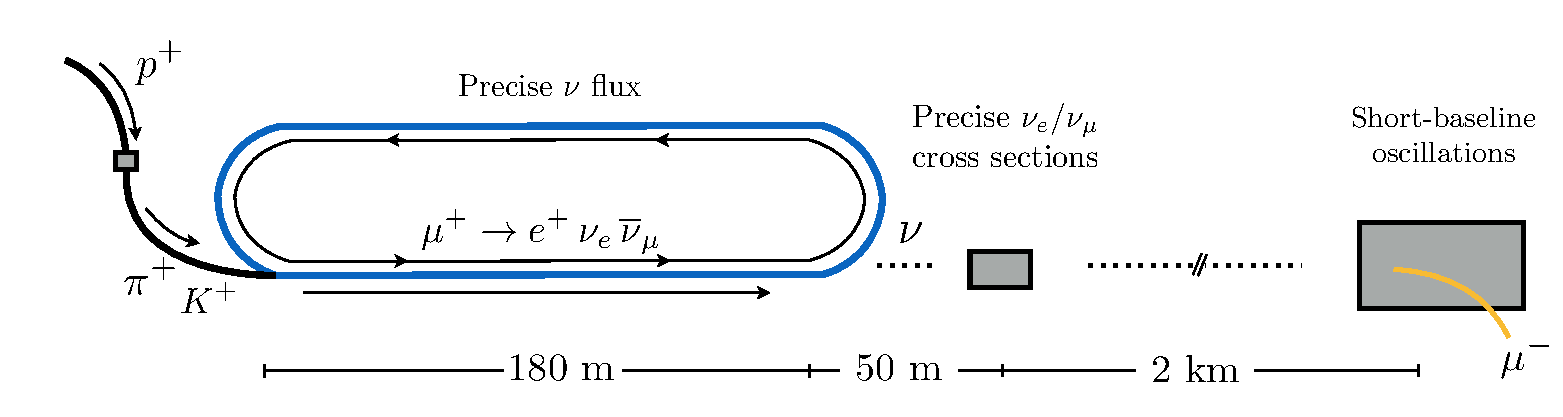
\includegraphics[width=\textwidth]{nustorm.pdf}
\caption[The \nus setup in a diagramatic representation.]{\nus in a diagram. \label{fig:nustorm_diagram}}
\end{figure}
%

The neutrino beam at \nus is derived from the decay of pions and stored muons. \nus is an accelerator neutrino experiment, and so relies on meson production in the usual way: high-energy protons colliding onto a solid target. A magnetic horn then collects $5.0 \pm 0.5$ GeV charged pions of the desired polarity, and inject them in the first straight of a racetrack like storage ring, where $52$\% of the collected charged pions are expected to decay before being stopped at the end of the straight. Muons with an energy of $3.8 \pm 0.38$ GeV are then collected and stored in the ring, where they are expected to circulate for a mean number of 50 turns. The first straight section of the ring, the decay pipeline, is estimated to be $180$ m long~\cite{Neuffer2015}, which will determine the size of the neutrino production region. 
In this setup, one obtains a beam of  $\nu_{\mu}$ ($\overline{\nu}_{\mu}$) from the decays of the injected $\pi^+$ ($\pi^-$) in what we call the \emph{pion flash}. The useful decays of the stored $\mu^+$ ($\mu^-$) then yield a beam of $\overline{\nu}_{\mu}$ ($\nu_{\mu}$) and $\nu_e$ ($\overline{\nu}_{e}$). The injection of pions into the ring is assumed to happen at large enough time intervals to allow for a discrimination between the neutrinos coming from the pion flash and the ones coming from the useful muon decays (a timing cut of the order of $180/c = 600$ ns or greater is needed to account for all pion decays before the muon data collection~\cite{Tunnell2013}). This allows us, for example, to completely separate the oscillations channels involving $\nu_{e}$ and $\overline{\nu}_{\mu}$ from the ones involving $\nu_{\mu}$ as initial states, for the $\pi^+$ polarity. It is clear, however, that a small contamination of muon decays happens during the pion flash. This is a small number of the neutrinos produced, and is taken into account by including $1\%$ of the muon decay flux into the pion flash neutrino flux. Kaons also contribute to the pion flash flux, albeit at larger energies. \reffig{fig:nustorm_flux} shows the neutrino flux at the near and far site, considered here.
%
\begin{figure}[t]
\centering
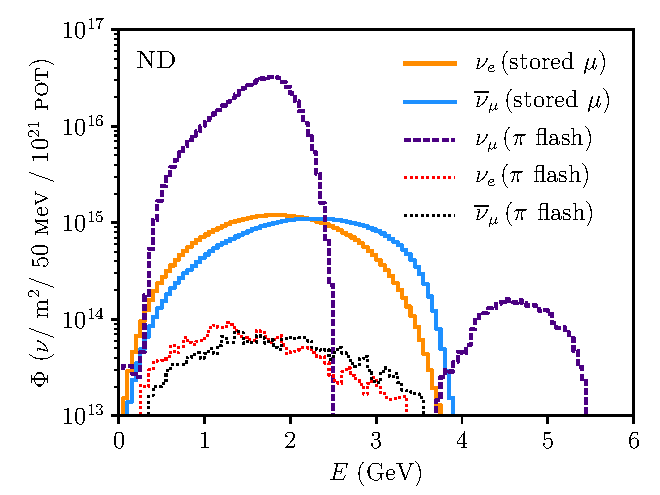
\includegraphics[width=0.49\textwidth]{figs/flux_ND.pdf}
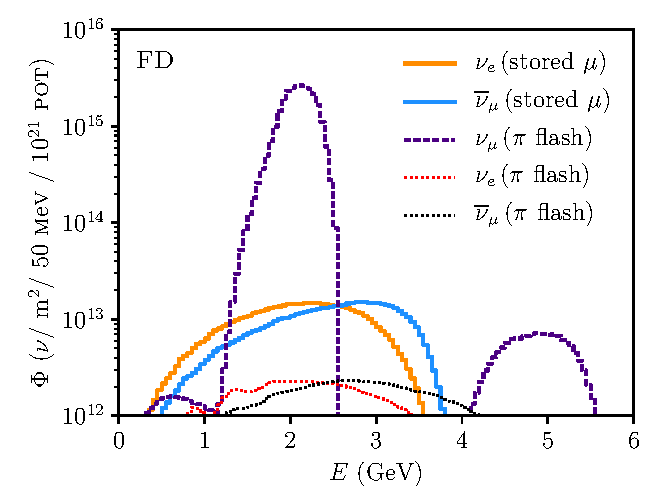
\includegraphics[width=0.49\textwidth]{figs/flux_FD.pdf}
\caption[The \nus neutrino flux for the near and far detector.]{The neutrino flux at the near (left) and far (right) detectors of $\nu$STORM. Note that the neutrinos from stored muons are separated from the ones generated in the pion flash through timing. \label{fig:nustorm_flux}}
\end{figure}
%

For the remainder of this section we present the results of our sensitivity studies for $\nu$STORM. We used the GLoBES package~\cite{Globes2005}, and implementing our own oscillation engine as well as our own treatment of the systematics. We start by noting that in an experiment like $\nu$STORM, the charge identification of muons is extremely important to separate neutrino and antineutrino events in the detectors. This is true independently of whether we are interested in oscillation analyses or cross section measurements. For instance, in an $\nu_{e} \to \nu_{\mu}$ appearance experiment, the greatest source of background comes from the misidentified intrinsic antineutrinos in the $\overline{\nu}_{\mu} \to \overline{\nu}_{\mu}$ channel. This, however, can be circumvented with large enough magnetic fields at the detectors and curvature analyses of the muon tracks. In all our simulations we assume that both the near and far detectors are magnetised. More specifically, we implement migration matrices for the SuperBIND style iron-scintillator detector, which have kindly been provided to us by the collaboration~\footnote{Ryan Bayes, private communication}. The far detector is assumed to have a fiducial mass of 1.3 kt, while the near detector is taken to be an identical but smaller version of the far detector with 0.2 kt of fiducial mass.

%
\renewcommand{\arraystretch}{1.2}
\begin{table}[h]
\begin{tabular}{lcc}
\hline
Sample&Channel& Sensitivity\\
%
\hline\hline
%
\multirow{2}{*}{$\pi^+$ flash} & $\nu_{\mu} \to \nu_{\mu} $ & $\sin^2{2\theta_{\mu\mu}}$ \\
%
\cline{2-3}
%
&$\nu_{\mu} \to \nu_{e}$&$\sin^2{2\theta_{e\mu}}$\\
 \hline
 %
 %
\multirow{3}{*}{Stored $\mu^+ $} & $\nu_{e} \to \nu_{e}$&$\sin^2{2\theta_{ee}}$\\
%
\cline{2-3}
%
&$\overline{\nu}_{\mu} \to \overline{\nu}_{\mu}$&$\sin^2{2\theta_{\mu\mu}}$\\
%
\cline{2-3}
%
&$\nu_{e} \to \nu_{\mu}$ & $\sin^2{2\theta_{e\mu}}$ \\
\hline
\end{tabular}
\caption[Oscillation channels at $\nu$STORM.]{The oscillation channels at $\nu$STORM, indicating to what phenomenological parameter they are sensitive to.\label{tab:nustorm_channels}}
\end{table}


We study various channels simultaneously at $\nu$STORM, however, only $\nu_\mu (\overline{\nu}_\mu)$ disappearance and $\nu_e \to \nu_\mu$ appearance count with existing migration matrices. For illustration, we also include oscillation channels involving electrons flavour in the final state. These will, of course, be challenging for iron detectors, but can become an additional goal if the detector are made of liquid Argon (LAr), for instance. For the current purposes, we take the analogous migration matrix with a muon in the final state, reduce the signal efficiency by a factor of $1/2$ and increase backgrounds by a factor of $400$. \reftab{tab:nustorm_channels} contains a summary of the signal channels we consider, and to which of the following phenomenological parameters they are sensitive to:
\begin{align}
 \sin^2{2\theta_{e\mu}} &= 4 |U_{e 4}|^2|U_{\mu 4}|^2,\nonumber\\ \sin^2{2\theta_{ee}} =  4|U_{e 4}|^2(1 -|U_{e 4}|^2), \quad&\quad \sin^2{2\theta_{\mu\mu}} =  4|U_{\mu 4}|^2(1 -|U_{\mu 4}|^2).
\end{align}



\subsection{Treatment of Systematics\label{sec:appendix_sys}}

Here, we detail our methodology for dealing with systematics errors at $\nu$STORM. We choose to use the pull method, which adds penalties to the best-fit parameter when deviating the parameters that control the systematics away from their central values. We work with a $\chi^2$ test which can be written as
%
\begin{equation}
\chi^2 _{\text{TOT}} = \sum_{D} \sum_{C} \chi^2_{D, C} + \chi^2_{\text{Pull}}.
\end{equation}
%
The $\chi^2_{D, C}$ for each detector $D$ and channel $C$ is a sum over the energy bins $E_i$ and a function of theoretical event rate $T^i_{D, C}$ and the simulated observed rate $O^i_{D, C}$:
%
\begin{equation}
\chi^2_{D, C} = 2 \sum_{i}^{n_{\text{bins}}} \Big(T^i_{D, C} - O^i_{D, C} + O^i_{D, C} \ln{\frac{O^i_{D, C}}{T^i_{D, C}}}\Big).
\end{equation}
%
The set of systematical errors for the signal and the background are represented by auxialiary parameters $\alpha$ and $\beta$, respectively, and are to be profiled over when calculating the theoretical event rates
%
\begin{align}
T^i_{D, C} =& (1 + \alpha_{\text{Flux}}^C + \alpha_{\text{Det}}^D + \alpha_{\text{Xsec}}^{i, C}) S^i_{D, C} + (1 + \beta^{D,C}) B^i_{D, C},
\end{align}
%
where $S^i_{D, C}$ and $B^i_{D, C}$ are the signal and background in the $i$-th energy bin, respectively. The error $\alpha_{\text{Flux}}^C$ is the total flux normalization error, correlated between near and far detector,  $\alpha_{\text{Det}}^D$ are the uncorrelated detector specific systematics and $\alpha_{\sigma_C}^i$ are the bin dependent cross sections and efficiency errors, which take shape uncertainties into account. We emphasize that the total flux normalization for the channels of interest is only uncorrelated between the two flux components. For examaple, for a $\pi^+$ polarity run, we have:
%
\begin{eqnarray}
\alpha_{\text{Flux}}^{\nu_{e} \to \nu_{\mu}} = \alpha_{\text{Flux}}^{\overline{\nu}_{\mu} \to \overline{\nu}_{\mu}} & =  \alpha_{\text{Flux}}^{\mu^+}, \quad  \alpha_{\text{Flux}}^{\nu_{\mu} \to \nu_{\mu}}  =  \alpha_{\text{Flux}}^{\pi^+}.
\end{eqnarray}
%
The background systematics take into account an overall normalization factor uncorrelated amongst all channels and detectors with $\beta_{BG}^{D,C}$ and shape effects with $\beta_{BG}^{i}$, also uncorrelated for all channels and detectors. Depending on what channel we are considering, there will be cross section uncertainties in the charge misidentificiation component of the background, which are taken into account in our analysis but not included in this discussion. In total, for our 4 channels of interest, 16 energy bins and one beam polarity, we have 52 signal systematic errors and 8 for the background.

In all our results, except when explicitly stated otherwise, we include 0.5\% flux normalisation uncertainties correlated between near and far detectors, and 0.5\% for detector specific uncertainties. Bin dependent cross section times efficiency uncertainties are taken to be 20\% at the time of the measurement, and overall background normalisation uncertainties 35\%. We also include an energy calibration error of 0.5\%. Finally, we point out that the $\chi^2$ analysis is done for the far and near detectors datasets separately, without resorting to near to far ratios.
 
\section{Sensitivity Results}

In the following sections we present our results for the sensitivity of \nus to different physical scenarios. 

\subsubsection{3+1 Oscillations}

In a 3+1 model, it is customary to present results in terms of the phenomenological parameters $\sin^2{2 \theta_{\alpha \beta}} = 4 |U_{\alpha 4}|^2|U_{\beta 4}|^2$ and $\sin^2{2 \theta_{\alpha \alpha}} = 4|U_{\alpha 4}|^2(1 - |U_{\alpha 4}|^2)$. \reffig{fig:3+1sens} shows the sensitivity of \nus to the phenomenological parameters in the 3+1 model, where the parametrization allows for a clear separation between appearance, $\nu_\mu$ disappearance and $\nu_e$ disappearance channels. We also show curves for single detector fits with and without systematics. For the combinations of both near and far detectors, we show the curve that would be obtained with a plane-wave treatment of oscillations, as well as the full localized oscillation probabilities. The latter represent our final results. 
%
\begin{figure}[t]
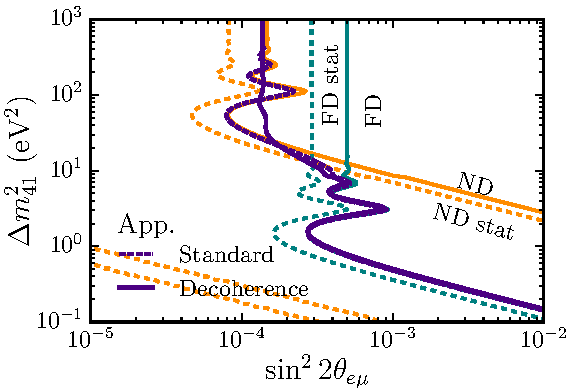
\includegraphics[width=0.49\textwidth]{figs/NDFD_Shape_app.pdf}
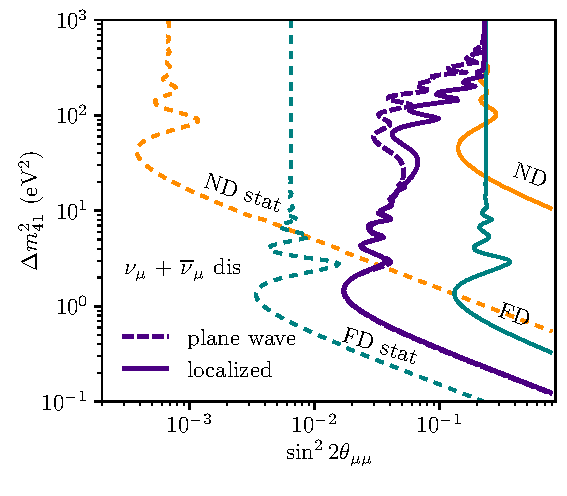
\includegraphics[width=0.49\textwidth]{figs/NDFD_Shape_dis.pdf}
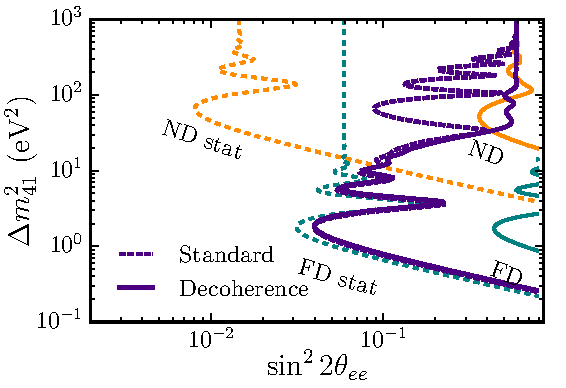
\includegraphics[width=0.49\textwidth]{figs/NDFD_Shape_edis.pdf}
\caption[The sensitivity of \nus to short-baseline oscillations in a 3+1 model.]{The $99\%$ C.L. sensitivities of \nus to the phenomenological parameters $\theta_{e \mu}$ (top left), $\theta_{\mu \mu}$ (top right), and $\theta_{ee}$ (bottom). The \textcolor{orange}{orange} (\textcolor{Cyan}{cyan}) curves assume only a single near (far) detector, respectively, and do not take localization into account. For those, dashed lines are the statistical limit. The dashed \textcolor{darkindigo}{purple} curves assume the presence of both detectors. Solid \textcolor{darkindigo}{purple} curves take localization into account.
\label{fig:3+1sens}}
\end{figure}
%

The interplay between the near and far detectors in this study is pivotal and has been discussed in the literature before in the context of the very low energy neutrino factory (VLENF)~\cite{Winter2012a}. For low $\Delta m^2_{41}$, the near detector is not affected by oscillations and can safely measure cross sections and detector efficiencies, while the far detector measures the oscillation parameters. The detector roles are swapped for larger $\Delta m^2_{41}$, however, where oscillations now develop at the near detector and are washed out at the far detector. In fact, due to localization effects, if $\Delta m^2_{41} \gtrsim 10$ eV$^2$, the oscillations are typically washed out at the near detector as well as at the far detector. In this case, the total effect is a constant shift of normalisation common between the near and far sites. This effect is less dramatic for $\nu_\mu$ disappearance as the pions are much shorter-lived. The production region, in this case, is $\ell_{{\rm dec}_\pi} \ll \ell_p = 180$ m, and so oscillations are localized for larger values of $\Delta m^2_{41}$. This effect is visible in \reffig{fig:3+1sens_v2}, where we show the $\nu_\mu$ disappearance sensitivity curves for the muon sample separately from that of the full sample (using neutrinos from pions as well as muon decays). \reffig{fig:3+1sens_v2} also shows the sensitivity obtained with our standard choice for systematics (20\% cross section $\times$ efficiencies, and $0.5\%$ correlated and uncorrelated flux uncertainties), as well as with a more pessimistic choice (35\% cross section $\times$ efficiencies, and $1\%$ correlated and uncorrelated flux uncertainties).


\begin{figure}[t]
\centering
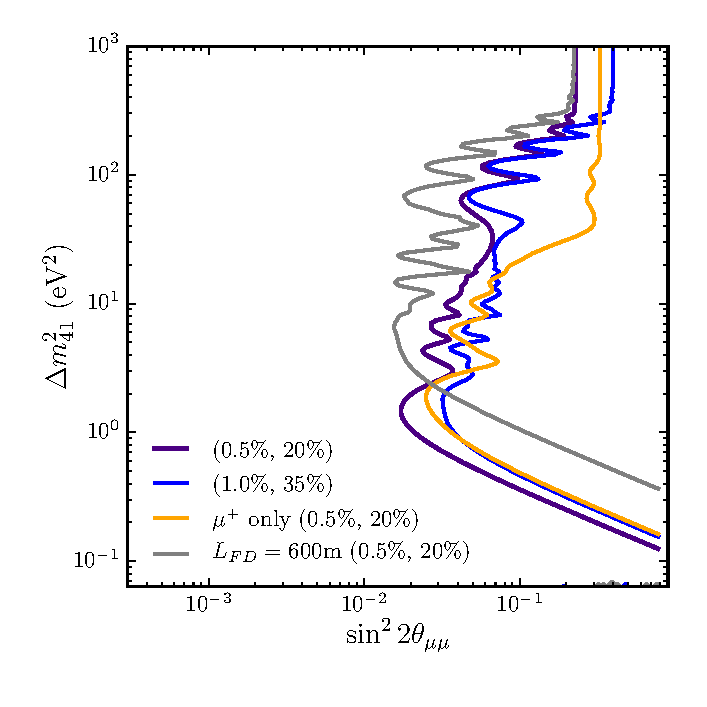
\includegraphics[width=0.49\textwidth]{figs/Comparison_dis.pdf}
\caption[Variations of the $\nu_\mu$ disappearance sensitivity.]{Variations of the $\nu_\mu$ disappearance sensitivity at $99\%$ C.L.. In \textcolor{darkindigo}{purple}, we show the main curve from \reffig{fig:3+1sens} and in \textcolor{blue}{blue} we increase all flux related systematic uncertainties to $1\%$ and cross sections $\times$ efficiencies uncertainties to $35\%$. With the standard systematics, in \textcolor{orange}{orange} we use only the events from stored muons (larger decay length).\label{fig:3+1sens_v2}}
\end{figure}
%
In \reffig{fig:all_bounds}, we compare \nus sensitivity curves to expected sensitivities for the SBN program~\cite{Cianci2017}, and overlay the existing bounds on the different active-heavy neutrino mixing. When plotting our results, we disregard bounds coming from astrophysical and cosmological observations (although these can be severe, especially at larger masses~\cite{Abazajian:2017tcc,Bridle:2016isd}). We also omit bounds from neutrinoless double-beta decay, which are model dependent and apply only if neutrinos are Majorana particles. In short, we display the strongest direct constraints on the existence of a fourth heavy neutrino from laboratory experiments. 

While an experiment like \nus is to test lower mass regions, it does perform much better than any other accelerator experiment for larger masses, where the measurement is essentially one of the zero-distance flavour transitions. As well as bounds from oscillation experiments, \reffig{fig:all_bounds} also shows bounds coming from $\beta$-decay experiments. These are obtained by searching for kinks in the kinematics of the outgoing electrons in beta decay. The curves shown are from Ref.~\cite{Dragoun2015} and correspond to the following radioactive isotopes: 1 -- $^3$H, 2 -- $^3$H, 3 -- $^{187}$Re, 4 -- $^3$H, 5 -- $^3$H, 6 -- $^{63}$Ni, 7 -- $^{63}$Ni, 8 -- $^{35}$S, 9 -- $^{64}$Cu, 10 -- $^{20}$F. The bound labelled 11 is from the Troitsk nu-mass experiment as reported in Ref.~\cite{Abdurashitov:2017kka}. Bounds on $|U_\mu4|^2$ come mainy from searches at IceCube~\cite{TheIceCubeCollaboration2016}, MINOS and MINOS+~\cite{Adamson:2017uda}~\footnote{This bound has generated debates in the literature and has been claimed to be too aggressive at large masses~\cite{Louis:2018yeg,Diaz:2019fwt}. In view of that, we hatch the relevant region in our plot.}. For $|U_{e4}||U_{\mu4}|$, we show bounds obtained from appearance experiments (electron-muon or muon-electron channels), where the NOMAD and CCFR curves were taken from Ref.~\cite{Astier2003}, and the NuTEV and KARMEN ones from Ref.~\cite{Avvakumov2002}.
%
Another way to bound the product of mixing elements is through the unitarity of the full mixing matrix. In fact, in any $3+N$ model, one can show that 
\begin{equation}
 P_{\alpha \to \beta} \leq \frac{1}{2} (1 - P_{\alpha \to \alpha})(1 - P_{\beta \to \beta}),
\end{equation}
or in terms of mixing matrix elements
\begin{equation}
\left( \sum_k 4 |U_{\alpha k}|^2|U_{\beta k}|^2 \right)^2 \leq \left( \sum_j 4 |U_{\alpha j}|^2( 1- |U_{\alpha j}|^2) \right)^2 \left( \sum_i 4 |U_{\beta i}|^2(1 - |U_{\beta i}|^2) \right)^2.
\end{equation}
This allows us to translate the bounds on $|U_{e 4}|$ and $|U_{\mu 4}|$ into bounds on the product $|U_{e 4} U_{\mu 4}|$, as we do in the bottom axes of \reffig{fig:all_bounds}.

\begin{figure}
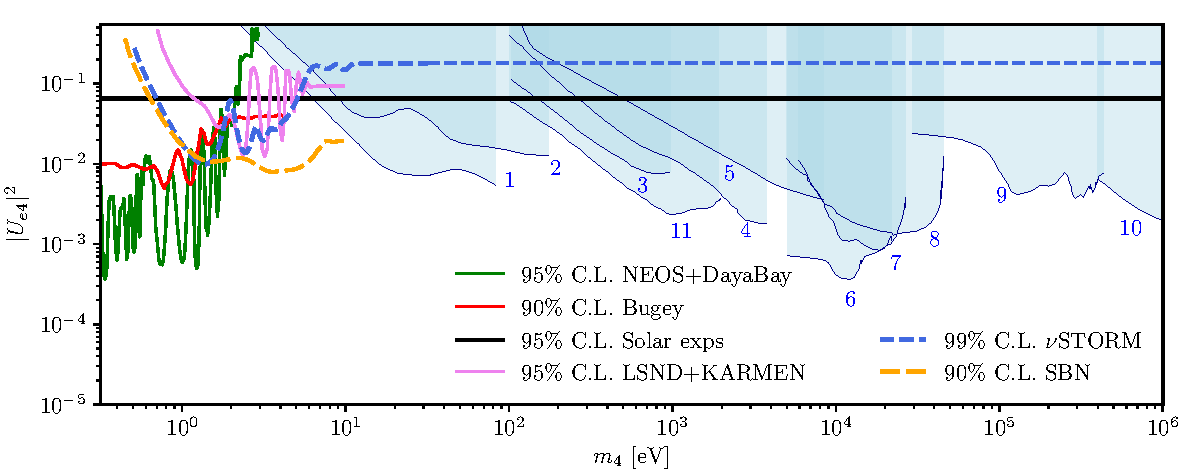
\includegraphics[width=\textwidth]{figs/Bounds_edis.pdf}
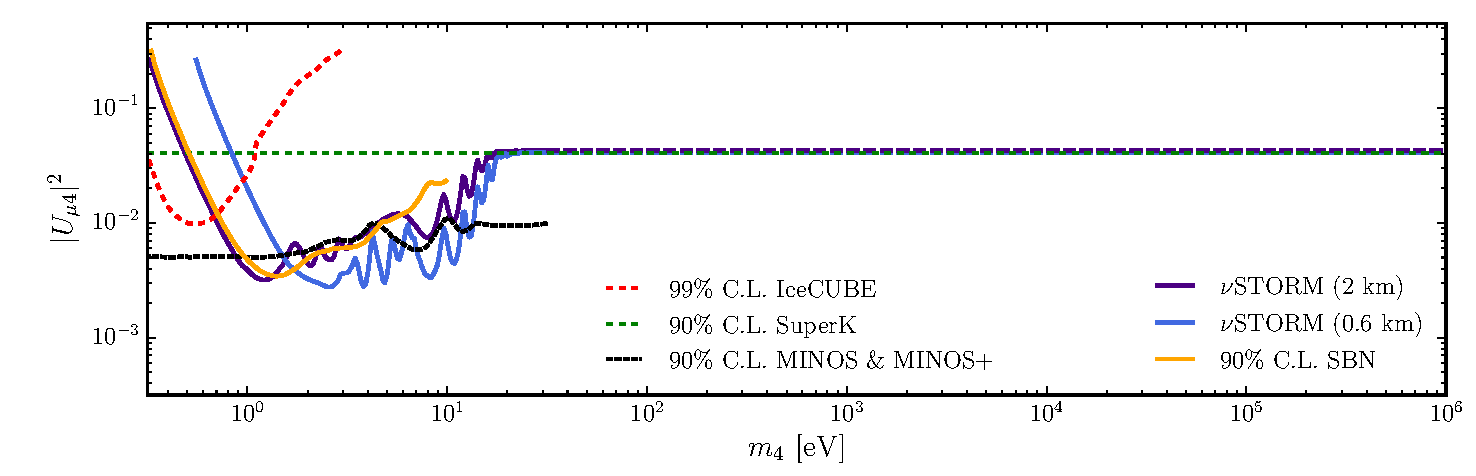
\includegraphics[width=\textwidth]{figs/Bounds_dis.pdf}
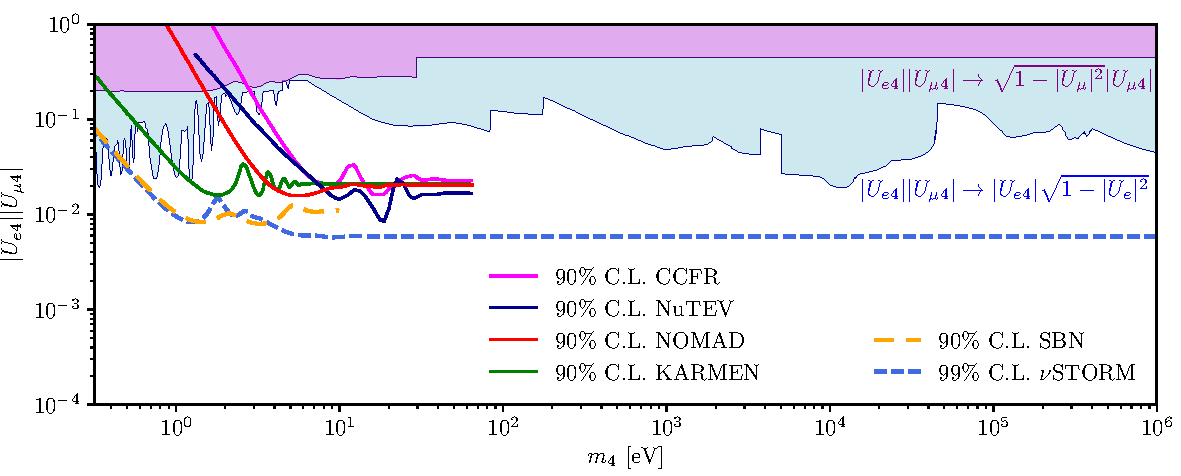
\includegraphics[width=\textwidth]{figs/Bounds_app_MH.pdf}
\caption[Laboratory bounds on active-heavy neutrino mixing in a 3+1 model.]{Laboratory bounds on the active-heavy mixing for the 3+1 model with $m_4 \approx \Delta m^2_{41}$. Constraints on mixing with electron flavour (top), muon flavour (middle), and the product of the two (bottom) are shown. The numbered bounds on $|U_{e4}|$ come from kink searches in $\beta$-decay and are all at 95\% C.L., except 2 and 9, which are at 90\% C.L. The projected sensitivities for SBN~\cite{Cianci2017} and $\nu$STORM shown as \textcolor{orange}{orange} and \textcolor{blue}{blue} dashed lines, respectively.\label{fig:all_bounds}}
\end{figure}


\subsubsection{3+2 Oscillations}

We now present our results for the 3+2 model. In this case, the ordering of the two sterile neutrinos is not physical, hence $\Delta m^2_{54} > 0 $ without any loss of generality. Note that now the presence of two oscillation frequencies complicates the interplay of the near and far detectors. If $\Delta m^2_{41}$ is in the $\mathcal{O}(1)$ ev$^2$ region and $\Delta m^2_{51}$ in the $\mathcal{O}(10^2)$ ev$^2$ region, then both the near and the far detectors are affected by flavour transitions and the systematics cannot be disentangled from the new physics effects in all cases.

A selected number of sensitivity curves in the 3+2 model are shown in figure \ref{fig:3+2sens_app}. We do not marginalise over the parameters that do not compose the axes, but rather set them to specific values. These are shown in the axes and were chosen based on the global-fit of Ref.~\cite{Collin2016a}, where the best fit is given by $\Delta m^2_{41} = 0.47 $ eV$^2$, $|U_{e4}|=0.13$, $|U_{e5}|=0.14$, $|U_{\mu4}|=0.15$, $|U_{\mu5}|=0.13$ and $\eta=-0.15\pi$.
%
\begin{figure}[t]
\centering
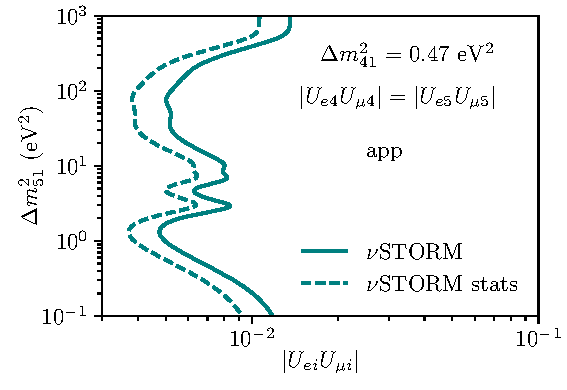
\includegraphics[width=0.49\textwidth]{figs/App_dm_UU.pdf}
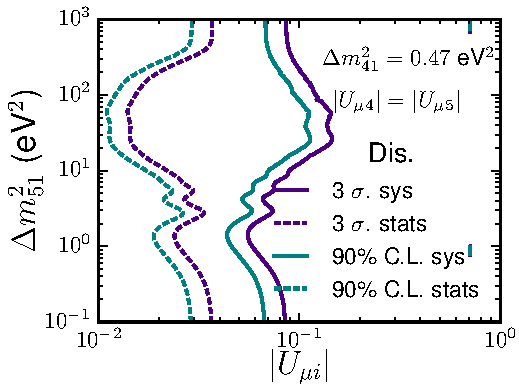
\includegraphics[width=0.49\textwidth]{figs/Dis_dm_UU.pdf}\\
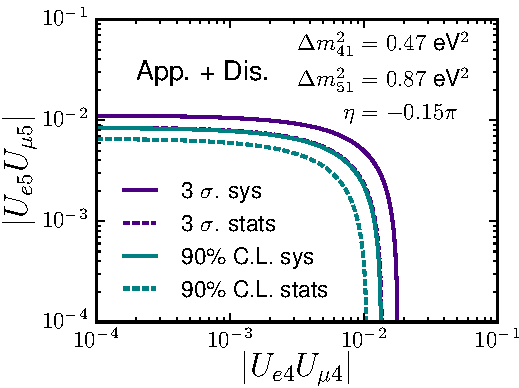
\includegraphics[width=0.49\textwidth]{figs/App_dm_UU_UU.pdf}
\caption[The sensitivity of \nus to short-baseline oscillations in a 3+2 model.]{The sensitivity of \nus to short-baseline oscillations in a 3+2 model at $99\%$ C.L. Top left shows the result of an appearance experiment, top right of a muon-disappearance experiment, and bottom of both channels combined.\label{fig:3+2sens_app} }
\end{figure}

Now, we assess the sensitivity of \nus to the effective short-baseline CP violation phase $\eta$ for a few choices of the 3+2 parameters. We repeat this study for different combinations of injected $\pi^+$ (stored $\mu^+$) and $\pi^-$ (stored $\mu^-$) modes, assuming the same efficiencies and fluxes for the CP conjugated channels.  Assuming a precision of 10\% and 20\% in the measurement of the 3+2 model parameters, we evaluate the sensitivity to $\eta$ in figure \ref{fig:CP1D}, showing that \nus could be sensitive to maximally CP violating phases at the 3 and 4 $\sigma$ level. This is to be contrasted with the study in Ref.~\cite{DeGouvea2015a}, where the CP violation arises from the interference between the $\Delta m^2_{31}$ and $\Delta m^2_{41}$ mass differences. Here, CP violation arises exclusively due to the interference between the two large oscillation frequencies.
%
\begin{figure}[t]
\centering
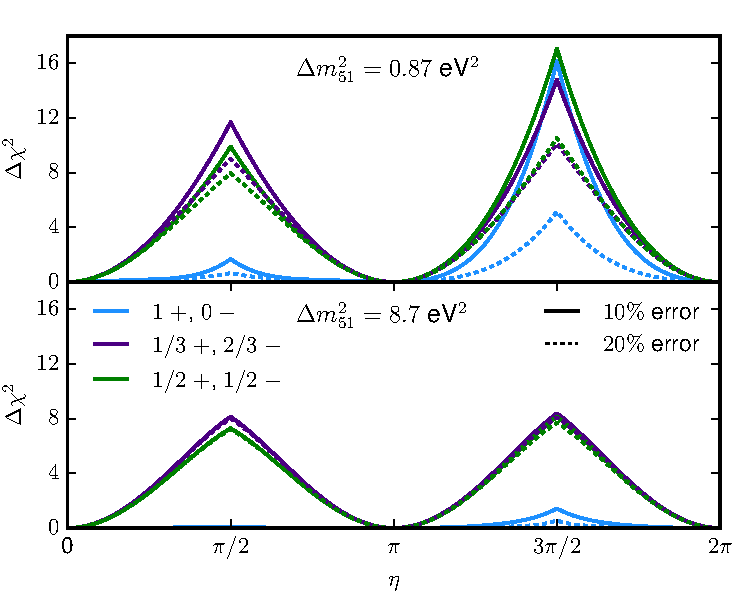
\includegraphics[width=0.49\textwidth]{figs/CP_sensitivity.pdf}
\caption[The sensitivity of \nus to short-baseline CP violation in a 3+2 model.]{The sensitivity of \nus to the CP violating phase $\eta$ when giving all other parameters $10 \%$ and $20 \%$ gaussian priors. The top axes show the choice of $\Delta m^2_{51} = 0.87 $ eV$^2$, while the bottom axes show a ten times larger value. We use three different configurations: 100\% $\mu^+$  runtime, 66\% $\mu^-$ and 33\% $\mu^+$ runtime, and 50\% runtime each. The other parameters in the 3+2 model are assumed to be $\Delta m^2_{41} = 0.47 $ eV$^2$, $|U_{e4}|=0.13$, $|U_{e5}|=0.14$, $|U_{\mu4}|=0.15$ and $|U_{\mu5}|=0.13$. \label{fig:CP1D}}
\end{figure}
%

\subsubsection{Averaged-out steriles}
  
Having discussed oscillations, we now focus on the flux normalization effects from averaged-out sterile neutrinos. This regime is already visible at large sterile masses in \reffig{fig:all_bounds}. Those bounds can be translated into model independent bounds on the sum of active-light neutrino mixing, as we do in this section. 

The zero-distance effects present in this averaged-out regime are hard to constrain in disappearance channels given the large cross section uncertainties, assumed to be $20\%$ here~\footnote{Improvements may come from restricting the analysis to well-known cross sections, such as $\nu-e$ scattering and neutrino-nucleus scattering with low $\nu = E_\nu - E_\ell$ values.}. For the $\nu_e\to\nu_\mu$ appearance channels, sensitivity is limited by backgrounds. These are typically small at \nus, since the final states contain muons, much easier to identify than electrons, and due to the presence a magnetic field to differentiate $\mu^+$ and $\mu^-$.

The results shown in \reffig{fig:non-uni} for $\nu$STORM are plotted compared with an existing study for MiniBoone~\cite{Karagiorgi2010} and SBN. We also show the bounds from  a global-fit to this type of non-unitarity in neutrino oscillations~\cite{Ross-Lonergan2016}.
%
\begin{figure}[t]
\centering 
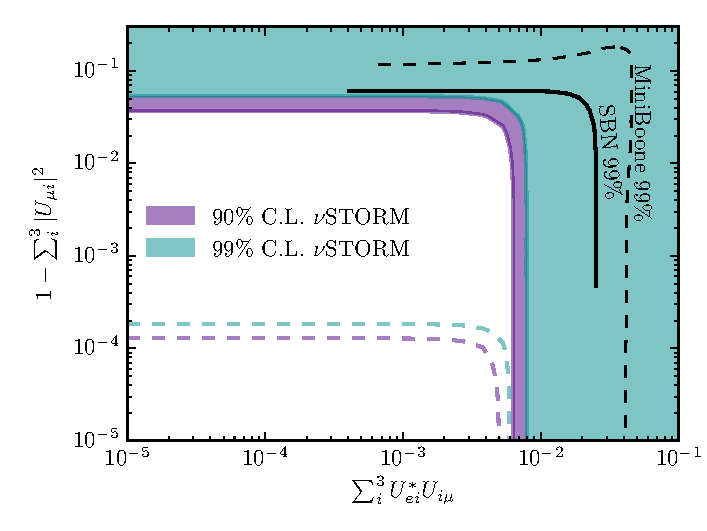
\includegraphics[width=0.49\textwidth]{figs/Averaged_joined.pdf}
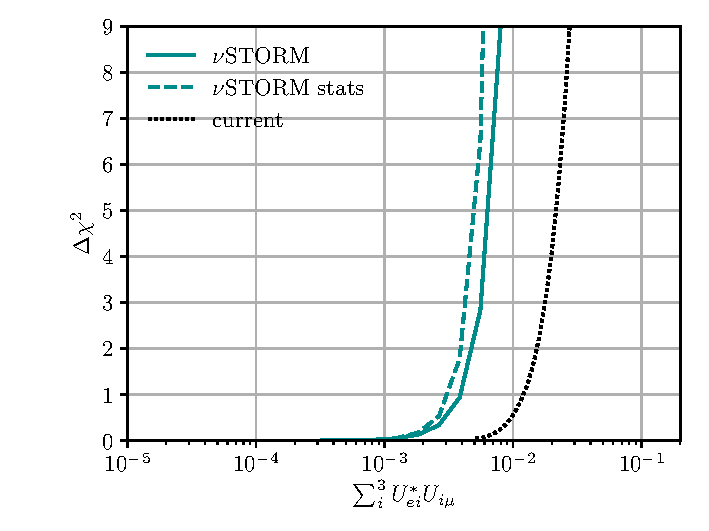
\includegraphics[width=0.49\textwidth]{figs/Averaged_1D_app.pdf}
\\
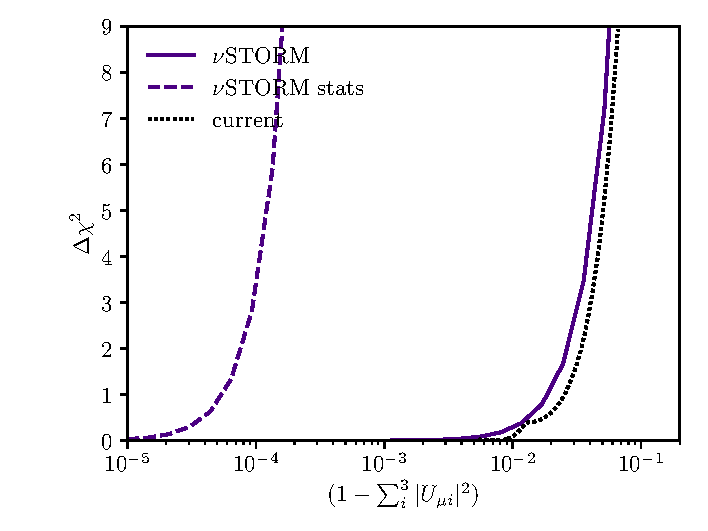
\includegraphics[width=0.49\textwidth]{figs/Averaged_1D_dis.pdf}
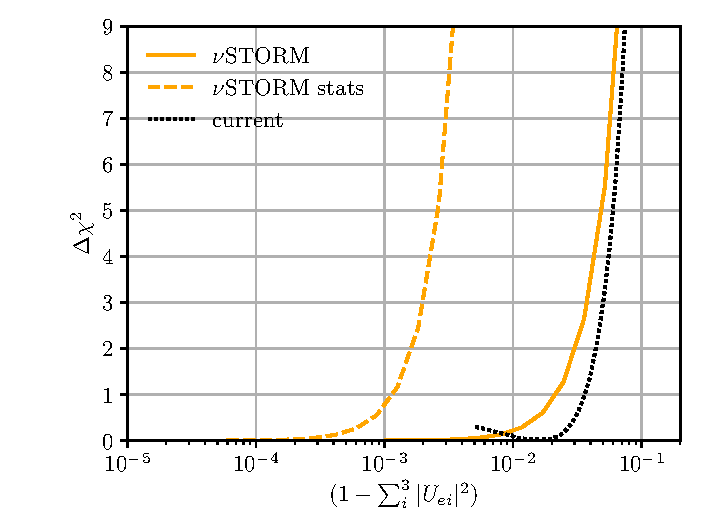
\includegraphics[width=0.49\textwidth]{figs/Averaged_1D_edis.pdf}
\caption[Bounds and sensitivity of $\nu$STORM to averaged out sterile neutrinos.]{Bounds on the non-unitarity of the mixing matrix in the averaged-out sterile case. Top left shows the two dimensional plane to which $\nu_\mu$ disappearance and $\nu_e \to \nu_\mu$ apperance experiments are sensitive to. We then show the one-dimensional $\Delta \chi^2$ profile for appearance (top right), $\nu_\mu$ disappearance (bottom left) and $\nu_e$ disappearance (bottom right). All colorful dashed lines stand for the statistical limit at $\nu$STORM.\label{fig:non-uni}}
\end{figure}
%

\subsubsection{Integrated-out steriles}

Now we show results for the integrated-out sterile at $\nu$STORM. For simplicity, we show our results in terms of a 3+1 parametrization, but the constraints can easily be translated into constraints on non-unitarity parameters (\eg, the $\alpha$ parameters). This is very similar to the averaged-out regime, however, different normalization factors appear in the oscillation probabilities depending on the production process of the intial neutrino. Let us emphasize that in the integrated-out regime, the different oscillation channels are now dependent on mixing matrix elements that may not even involve the neutrino (low energy) flavours. In fact, the channels $\nu_{\mu} \to \nu_{\mu}$ and $\overline{\nu}_{\mu} \to \overline{\nu}_{\mu}$ depend on different mixings, since they involve neutrinos with different parent particles.
%
\begin{figure}
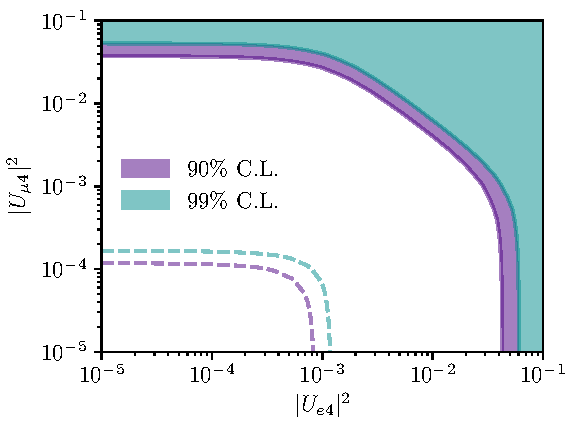
\includegraphics[width=0.48\textwidth]{figs/MUV_joined.pdf}
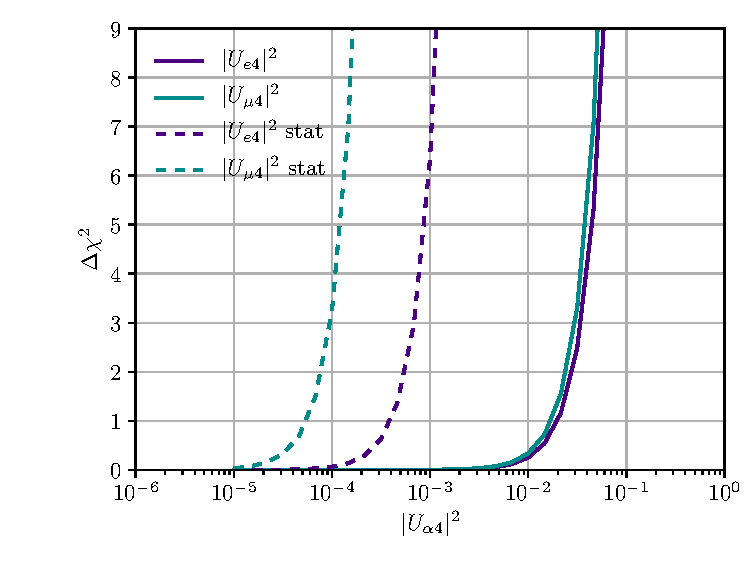
\includegraphics[width=0.49\textwidth]{figs/MUV_1D.pdf}
\caption[Sensitivity to non-unitarity in the integrated-out sterile case.]{Sensitivity to non-unitarity in the integrated-out sterile case. Dashed lines stand for the statistical limit at $\nu$STORM. \label{fig:non-uni_MUV}}
\end{figure}
%
In our implementation, we define an effective flavour transition probability $\hat{P}$ which absorbs any factors due to non-unitarity at production and detection
%
\begin{equation}
 \hat{P}_{\nu_{\alpha} \to \nu_{\beta}} = \frac{\sigma^{\text{CC}}_{\alpha}}{\sigma^{\text{CC (SM)}}_{\alpha}} \, P_{\nu_{\alpha} \to \nu_{\beta}} \, \frac{d\Phi^{\text{CC}}_{\alpha}/dE}{d\Phi^{\text{CC (SM)}}_{\alpha}/dE},
\end{equation}
where $P_{\nu_{\alpha} \to \nu_{\beta}}$ is the standard probability. The explicit expressions we use in this analysis are shown below for the different samples.
\begin{itemize}
 \item \underline{$\pi^+ (k^+) \to \mu^+ \nu_{\mu}$:}
      \begin{align}
	\hat{P}_{\nu_{\mu} \to \nu_{\mu}} &= 1 - 2 |U_{\mu 4}|^2 + |U_{\mu 4}|^4, \\
	\hat{P}_{\nu_{\mu} \to \nu_{e}} &= |U_{e 4}|^2|U_{\mu 4}|^2.
      \end{align}
 \item \underline{$\mu^+ \to e^+ \nu_{e} \overline{\nu}_{\mu}$:}
      \begin{align}
	\hat{P}_{\nu_{e} \to \nu_{e}} &= \left(1 - 2 |U_{e 4}|^2 + |U_{e 4}|^4\right) \left( 1 - |U_{\mu4}|^2\right), \\	
	\hat{P}_{\overline{\nu}_{\mu} \to \overline{\nu}_{\mu}} &= \left(1 - 2 |U_{\mu 4}|^2 + |U_{\mu 4}|^4\right) \left( 1 - |U_{e4}|^2\right), \\
	\hat{P}_{\nu_{e} \to \nu_{\mu}} &= |U_{e 4}|^2|U_{\mu 4}|^2\left( 1 - |U_{\mu4}|^2\right).
      \end{align}
\end{itemize}
%
The bounds that \nus could place on neutrino mixing in this regime are shown in Fig.~\ref{fig:non-uni_MUV}. Although \nus possesses the advantage of a precise flux, the bound in this regime are much less competitive with bounds obtained from the charged-lepton sector. For instance, precision measurements in the charged-lepton and quark sectors yield a bound on $|U_{\mu4}|<0.021$ at $2\sigma$~\cite{Fernandez-Martinez:2016lgt}. This is to be contrasted with the $\nu$STORM sensitivity to $|U_{\mu4`}|>0.19$ at $2\sigma$. The situation is much worse for the product $|U_{e4} U_{\mu4}|$. There, $|U_{e4} U_{\mu4}|<2.4\times10^{-5}$ due to lepton flavour violation bounds (dominated by $\mu\to e \gamma$ searches), while $\nu$STORM is only sensitive to $|U_{e4}U_{\mu4}| > 6.4\times 10^{-3}$. 

\section{Overview}

The novel neutrino beam at \nus allows for interesting possibilities in the search for short-baseline oscillations. Despite the precise flux, cross section and efficiency uncertainties still greatly limit the power of any disappearance search, especially for constant flavour transitions. The possibilities considered here, however, are not exhaustive. In view of the redesign of the proposal for siting at CERN, this work can be adapted to higher neutrino energies and different detector materials. In particular, opting for (magnetized) LAr detectors, would allow to explore all oscillation channels available at \nus to the fullest. Other great improvements on searching for new physics can be achieved by combining well-known cross sections with the well-known flux at $\nu$STORM. As a next step, we envisage applying the same study to neutrino-electron scattering for different detector choices. Measuring this process is currently a method to obtain information on the neutrino flux at accelerator experiments, since its cross sections is well known. At $\nu$STORM, it can be used to constrain new physics since the cross section uncertainties would be reduced from tens of a percent to the few percent level. Sterile neutrinos and non-unitarity need not be the only goal of such analyses. Precision measurements of electroweak parameters, such as $\theta_\textsc{w}$, can also be achieved through these methods. The limitation, however, lies mainly on the statistics and detector performance. 

Other avenues to precise GeV neutrino beams also exist. For instance, the \textsc{enubet} proposal~\cite{Acerbi:2645532,Acerbi:2019qiv}, where a well-understood $\nu_e$ beam is obtained from decays of the type $K^+\to \pi^0 e^+ \nu_e$. In this way, the proposal aims to tag each neutrino interaction in the detector with a particular daughter lepton at production, promising the first tagged neutrino beam. At higher energies, above tens of GeV, the neutrino DIS cross sections offer better precision and higher rates, although also relying on our ability to understand the flux. 

